\documentclass{ctexrep}
\usepackage{graphicx}


\begin{document}
\title{高斯混合模型(GMM)和EM算法}
\maketitle


	
%高斯混合模型简介
\section{高斯混合模型}

高斯混合模型,是由多个高斯分布混合形成的分布,可以由下式表示:
$$P(X|\theta)=\sum_{k=1}^K{w_kf(X|\theta_k)}$$
其中$\theta_k=(\mu_k,\sigma_k)$,$f(X|\theta_k)=N(\mu_k,\sigma_k)$.

一般,一个简单的概率分布可以根据\emph{观测数据}X,使用\emph{极大似然估计}估算该分布概率的参数$\theta$.\footnote{思路是:若采集到了观测数据X,则认定这组观测数据出现的概率在客观上是最大的;客观上出现概率小的数据不容易被观测到.这样,可以假定一个概率分布模型,以该分布模型的参数$\theta$为变量,进行最优化,使得观测数据对应的概率最大,则该$\theta$,为观测数据的极大似然估计\cite{概率论-茆}.}
$$\hat{\theta}=\arg\max L(\theta)$$

但是由于高斯混合模型含有\emph{隐变量}$w_k$,所以使用极大似然估计没有解析解,只能通过迭代方法求解.

\paragraph{隐变量}
关于隐变量,可以使用三硬币模型说明.\cite{统计学习方法}

其过程是:先抛硬币甲,1)如果硬币甲是正面(事件$z_1$),则抛硬币乙,并将乙的结果当作最终观测数据;2)如果硬币甲是反面(事件$z_2$),则抛硬币丙,并将丙的结果当作最终观测数据.

\begin{figure}[hbt]
	\centering
	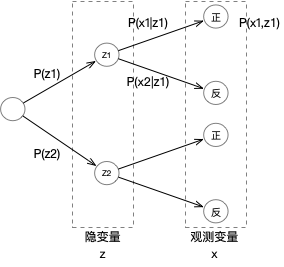
\includegraphics[width=.5\linewidth]{三硬币示意图.png}
	\caption{三硬币模型}
	\label{三硬币模型}
\end{figure}





%简述EM算法流程及证明
\section{EM算法}

%算法流程
\paragraph{算法流程}
\begin{enumerate}
	\item 选取初值$\theta^{0}$.
	\item E步:$$Q(\theta,\theta^{i})=\sum_z P(Z|X,\theta^{i})\log{P(X,Z|\theta)}$$
	\item M步:$$\theta^{i+1}=\arg\max Q(\theta,\theta^{i+1})$$
\end{enumerate}

%原理及证明
\paragraph{原理及证明}
首先将似然函数\cite{概率论-茆}$L(\theta)$改写成$\theta$和$z$的函数$L(\theta,z)$.

似然函数为\footnote{$ L(\theta) = \log\prod\limits_iP(x^i|\theta)= \sum\limits_{i} logP(x^i|\theta) $}
$$L(\theta)=\sum_i \log P(x^i|\theta) $$

\begin{equation}
	L(\theta)=\sum\limits_i\log{P(x^i|\theta)}
	=\sum\limits_i\log{ \sum\limits_j{P(x^i,z^j|\theta)}}
\end{equation}

将最右端的隐变量$z$和观测变量$x$的联合概率,用隐变量$z$的条件概率表示\footnote{$P(x,z|\theta)=P(z)P(x|z,\theta)$}

故
\begin{equation}
	L(\theta,z)=\sum\limits_i{ \log \sum\limits_j{ P(z^j)\frac{P(x^i,z^j|\theta)}{P(z^j)}}}
\end{equation}

\paragraph{Jensen不等式}\footnote{虽然表述为期望$E[]$,但理解成\emph{均值定理}的推广更为合适,如式3.}

如果$f(x)$为凸函数,则有$E[f(x)] \geq f[E(X)]$.

简单证明:\\
对于任意点集${x_i},i=1,..M$,且$\lambda_i\geq0$,$\sum\limits_{i=1}^M{\lambda_i}=1$.\\当$M=2$时,如图2所示,有$\lambda_1f(x_1)+\lambda_2f(x_2)\geq f(\lambda_1x_1+\lambda_2x_2)$\\
显而易见,当$M=\infty$时,
\begin{equation}
	\sum\limits_i{\lambda_if(x_i)}\geq f(\sum\limits_i \lambda_ix_i)
\end{equation}

即$$E[f(x)] \geq f[E(X)]$$

当$x_1=x_2=x_3...x_M$时,等号成立.即$\sum\limits_i{\lambda_if(x_i)}=f(\sum\limits_i \lambda_ix_i)$.


\begin{figure}[hbt]
	\centering
	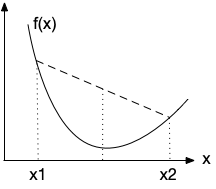
\includegraphics[width=.3\linewidth]{凸函数.png}
	\caption{Jensen不等式}
\end{figure}

接式2,$\log$函数(底$>1$时)为凹函数.有$\sum\limits_i{\lambda_i\log(x_i)}\leq \log(\sum\limits_i \lambda_ix_i)$.所以有:
\begin{equation}
	L(\theta,z)
	=\sum\limits_i{ \log \sum\limits_j{ P(z^j)\frac{P(x^i,z^j|\theta)}{P(z^j)}}}
	\geq \sum\limits_i{ \sum\limits_j{ P(z^j)\log{\frac{P(x^i,z^j|\theta)}{P(z^j)}}}}
\label{ltz_j}
\end{equation}

上式右端为$L(\theta,z)$的下界.这里通过极大化式4下界的方法求解极大化$L(\theta,z)$.

\paragraph{极大化似然函数下界}
当$\frac{P(x^i,z^j|\theta)}{P(z^j)}$等于某常数时,式4等号成立,即下界最大.
此时有
$$\frac{P(x^i,z^j|\theta)}{P(z^j)} = c$$
$$\sum\limits_j P(z^j) = 1$$

所以有$$\sum\limits_j P(x^i,z^j|\theta)=c$$
\begin{equation}
	P(z^j)=\frac{P(x^i,z^j|\theta)}{c}=\frac{P(x^i,z^j|\theta)}{\sum\limits_j P(x^i,z^j|\theta)}=P(z^j|x^i,\theta)
\label{pz}
\end{equation}
此时下界最大.

至此,便实现利用Jensen不等式求出$L(\theta,z)$的下界,并求出令下界最大的$P(z^j)$的取值:$P(z^j)=P(z^j|x^i,\theta)=\frac{P(x^i,z^j)}{\sum\limits_j{P(x^i,z^j)}}$.如图\ref{简化三硬币模型}

由图\ref{三硬币模型}所示,此时已经将隐变量已不再是变量,可以当作常量,化简分布模型.

\begin{figure}[hbt]
	\centering
  	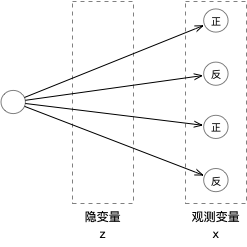
\includegraphics[width=0.4\linewidth]{三硬币化简示意图.png}
  	\caption{简化三硬币模型}
  	\label{简化三硬币模型}
\end{figure}


将式\ref{pz}代回式\ref{ltz_j},有
\begin{equation}
	L(\theta)
	=\sum\limits_i\sum\limits_j P(z^j|x^i,\theta)\log P(x^i,z^j|\theta)-\sum\limits_i\sum\limits_j P(z^j|x^i,\theta)\log P(z^j|x^i,\theta)
\label{5->4}
\end{equation}
即$$L(\theta)=\sum\limits_i\sum\limits_j P(z^j)\log P(x^i,z^j|\theta)=E_z[P(X,Z|\theta)]_{|
X,\theta}=Q(\theta)$$

上式\ref{5->4}右端第二项,是$P(z^j|x^i,\theta)$的函数,为常量,在极大化$L(\theta)$时可以忽略.上式便是算法步骤中的E步.

至此,便可以使用常规办法求解$\hat{\theta}=\arg\max{L(\theta)}$.这里便是算法步骤中的M步.

\paragraph{总结}
先假定初值$(z^0,\theta^0)$,带入到E步公式求解出$Q$函数.$Q$函数为调整$z$能获得的最大值.再对$Q$函数求最大值,调整$\theta$.反复迭代上述过程,直至收敛,获得$(\hat{z},\hat{\theta})$.










\bibliographystyle{plain}
\bibliography{refs.bib}



\end{document}